\documentclass{article}
\usepackage{graphicx}
\usepackage{booktabs}
\usepackage{multirow}
\usepackage{amsmath}
\usepackage{float}
\usepackage{placeins}
\usepackage{array}     % For better column control
\usepackage{geometry}
% Required packages (add to preamble)
\usepackage{fancyhdr}  % For header/footer styling
\usepackage{setspace}  % For line spacing
\usepackage{makeidx}  
\usepackage[nottoc]{tocbibind} % Adds References to TOC
\usepackage[utf8]{inputenc}
\usepackage{textgreek} % for Greek letters in text
\makeindex                  % Initializes index
\geometry{a4paper, margin=1in}


% Page formatting
\addtolength{\textwidth}{5mm}
\addtolength{\textheight}{12mm}
\addtolength{\topmargin}{-10mm}
\pretolerance = 10000000
\setlength{\parindent}{0pt}
\setlength{\parskip}{\baselineskip}
\onehalfspacing   
 
% Header / footer
\pagestyle{fancy}
\lhead{Manvendra Kumar Mishra, 2019011048}
\chead{}
\rhead{\em MATH5747M, Assignment 4}
\lfoot{}
\cfoot{\thepage}
\rfoot{}
\setlength{\headheight}{20pt}
\renewcommand{\headrulewidth}{0.4pt}
\renewcommand{\footrulewidth}{0pt}


\title{Cancer and Socioeconomic Disparities: An Analysis of Deprivation Effects Using NHS Simulacrum Data}
\author{Manvendra Kumar Mishra}
\date{\today}

\begin{document}

\begin{titlepage}

    \centering
    \vspace*{\fill} % Fills vertical space above
    
        \begin{figure}[H]
        \centering
        \includegraphics[width=0.2\linewidth]{uni_logo.jpeg}
        \label{fig:enter-label}
    \end{figure}

    {\LARGE\bfseries Investigating Cancer Cases In UK Population\par}
    {\LARGE\bfseries Cancer and Socioeconomic Disparities\par}
    \vspace{0.5cm}
    {\large An Analysis of Deprivation Effects Using NHS Simulacrum Data\par}
    
    \vspace{1cm}
    {\large Manvendra Kumar Mishra\par}
    
    \vspace{1cm}
    {\large \today\par}
    
    \vspace*{\fill} % Fills vertical space below
\end{titlepage}

\clearpage
\tableofcontents
\clearpage
% ------------Introduction Section -----------------

\section{Introduction}
In the current world, cancer has become a leading cause of morbidity and mortality, with socioeconomic disparities significantly influencing incidence, diagnosis, treatment and survival outcomes \cite{Siegel2023}. In the United Kingdom, the NHS plays a leading role in the treatment of these diseases, and the Simulacrum dataset provided by the NHS gives valuable insights about such issues by linking the registered cancer patients with their demographic and deprivation indices.

% \vspace{0.3cm} % Vertical space after the paragraph

The unit ``Deprivation'' is measured by the Index of Multiple Deprivation quantiles (\texttt{QUANTILE\_2019}) in dataset. This unit is a critical factor while talking about health inequities, based on the status and with prior research indicates more cancer cases and poorer outcomes in various deprived populations \cite{CancerResearchUK2022}. 

% \vspace{0.3cm} % Vertical space after the paragraph

This report analyses the relationship between cancer type and deprivation level across age categories and gender, and explores the survival rate and treatment duration to identify the mentioned key disparities. Below are the focus areas of this report:

\begin{itemize}
    \item Whether a certain cancer type is more prevalent in any deprived area.\cite{Lyratzopoulos2013}
    \item How age plays a role in the deprivation quintiles.
    \item Whether survival rate differs by socioeconomic status for specific cancers \cite{Coleman2011}
    \item Role of certain gender in moderating the deprivation-cancer relationship.
    \item Feasibility in predicting deprivation level using the Simulacrum patient-level dataset.
\end{itemize}

By using statistical and machine learning modeling techniques, this report aims to analyze and inform targeted public health interventions to reduce cancer inequities in the UK population.


% ------------Data Overview Section -----------------


\section{Data Overview}
This report is based on the NHS Simulacrum cancer dataset \cite{NHSDigital2023}, a synthetic dataset designed to mimic real-world cancer registrations while preserving patient confidentiality. The dataset is distributed across multiple tables, containing records of cancer patients along with their associated demographic, socioeconomic, and clinical variables.


\subsection{Key Variables}
The dataset includes the following key variables:

\begin{itemize}
    \item \textbf{Patient IDs:} Each record corresponds to a single patient, with unique registration numbers serving as patient identifiers.
    
    \item \textbf{Cancer Type:} Represented in a coded structure following the ICD-10 classification (e.g., \texttt{C34} for Lung Cancer).
    
    \item \textbf{Deprivation Level:} Measured using the Index of Multiple Deprivation (IMD), stored in the column \texttt{QUANTILE\_2019}.
    
    \item \textbf{Age at Diagnosis:} Provided either as a continuous variable or in binned age groups, available in the \texttt{AGE} column.
    
    \item \textbf{Gender:} Primarily includes \texttt{Male} and \texttt{Female} categories.
    
    \item \textbf{Survival Status:} Encoded to indicate patient outcomes such as \texttt{Alive}, \texttt{Deceased}, or as time-to-event data.
    
    \item \textbf{Treatment Duration:} The length of treatment received by the patient.
\end{itemize}

\subsection{Data Sanity Checks}
The following data quality checks were performed to ensure the reliability of the analysis:

\begin{itemize}
    \item \textbf{Missing Data Exclusion:} 
    Records with no or null values in \texttt{CancerType} or \texttt{QUANTILE\_2019} fields were excluded from the analysis.
    
    \vspace{0.2cm}
    
    \item \textbf{Age Validation:} 
    Extreme age values (e.g., \texttt{age < 18} or \texttt{age > 100}) were reviewed for plausibility and either corrected or excluded when implausible.
    
    \vspace{0.2cm}
    
    \item \textbf{ICD-10 Code Verification:} 
    All cancer type codes were cross-checked against the official NHS ICD-10 classification to ensure validity.
\end{itemize}



\subsection{Initial Insights}
The analysis utilizes two primary datasets from the NHS Simulacrum: \texttt{sim\_av\_patient} and \texttt{sim\_av\_tumour}. Below are the initial insights on the datasets used: 

\begin{itemize}
    \item \textbf{\texttt{sim\_av\_patient}}: 
    Contains patient demographic information. The raw dataset includes:
    \begin{itemize}
        \item 12 columns of patient attributes
        \item 1,871,605 patient registration records
    \end{itemize}
    
    
    \item \textbf{\texttt{sim\_av\_tumour}}: 
    Provides socioeconomic and diagnostic information. The raw dataset contains:
    \begin{itemize}
        \item 37 columns of patient-level variables
        \item 1,995,570 rows of tumor-level records
    \end{itemize}

    \item There are 109 different types of cancer data present in the merged file.
    \item The age group in the raw data varies from minimum of age 0 and maximum of 107 years old, with total number of 729 records having age of 0 years. Which is removed during pre-processing.
\end{itemize}


% ------------EDA Section -----------------

\section{Exploratory Data Analysis}
In this section we will explore the data to find out any initial patterns in the dataset corresponds to different variables and factors like cancer incidents, demographic and socioeconomic disparities and their relationship with the cancer cases using various visualization techniques and any descriptive statistics if required. Also, the key focus will be to include age/gender distributions, deprivation based factors and any related trends if present in the data before we move to the modeling part.

% \vspace{0.3cm} % Vertical space after the paragraph

[Note]: Additionally, as there are 109 different cancer types present in the data. Our main focus is to analyze top 10 cancer types based on the patient counts, to minimize the cleanliness and prioritize the major concern areas.

\subsection{Cancer Type Distribution}
Figure \ref{fig:cancer_freq} shows the frequency distribution of different cancer types .Below are the key observations based on the distribution (bar) chart:
\begin{itemize}
    \item Breast and prostate cancers are the most prevalent in the dataset
    \item There is a significant drop-off after the top three cancer types (breast, prostate, lung)
    \item Rare cancers like kidney (27,325 cases) appear at the lower end of the spectrum
\end{itemize}


\begin{figure}[H]
    \centering \fbox{
    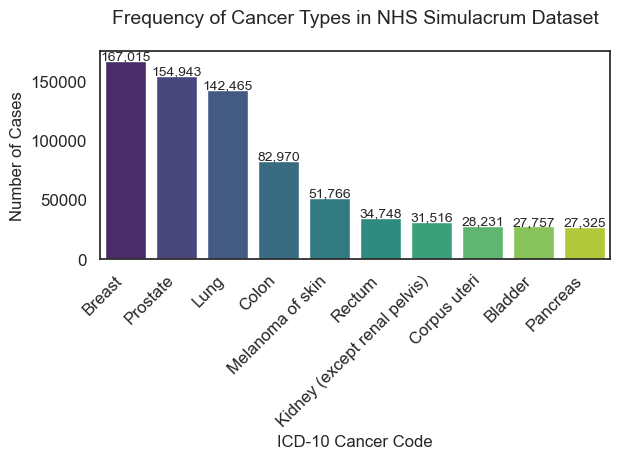
\includegraphics[width=0.8\textwidth]{Freq_Of_Cancer_Types.png}}
    \caption{Frequency of Cancer Types (Top 10)}
        \label{fig:cancer_freq}
\end{figure}


The bar chart shows the number of cases for each cancer type (top 10), with breast cancer showing the highest number of cases (152,015 cases), followed by prostate cancer (154,943 cases) and lung cancer (142,465 cases).

\subsection{Deprivation Analysis}
\begin{figure}[H]
    \centering\fbox{
    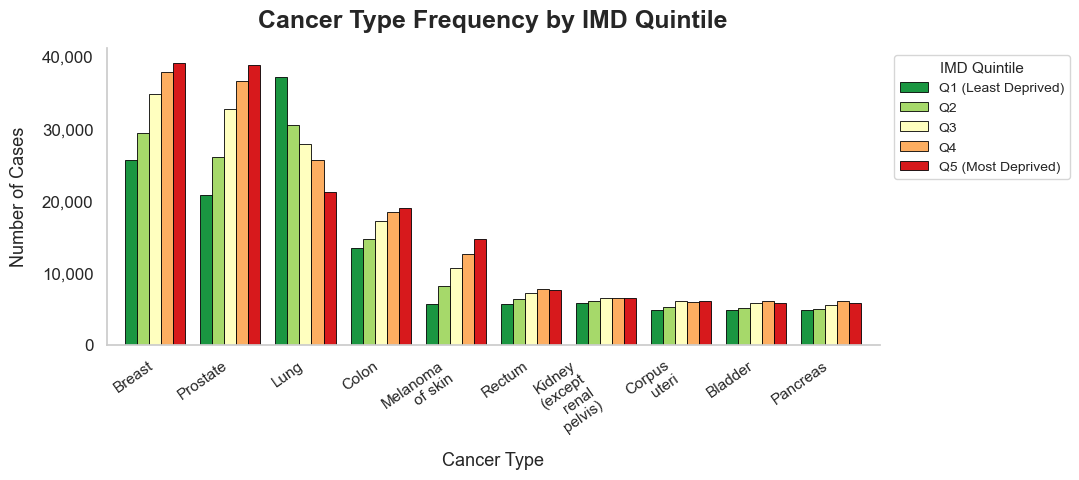
\includegraphics[width=0.9\textwidth]{Cancer_Type_Frequency_by_IMD_Quintile.png}
    }
    \caption{Cancer Frequency by Deprivation Level}
    \label{fig:imd_analysis}
\end{figure}

Figure \ref{fig:imd_analysis} reveals significant variation in cancer prevalence across deprivation quintiles:

\begin{itemize}
    \item \textbf{Breast cancer} shows higher incidence in less deprived quintiles (Q1-Q2)
    \item \textbf{Lung cancer} demonstrates a strong deprivation gradient, with Q5 (most deprived) having 2.3$\times$ more cases than Q1
    \item \textbf{Prostate cancer} maintains relatively stable rates across quintiles
    \item \textbf{Melanoma} follows an inverse deprivation pattern, with Q1 showing 68\% higher incidence than Q5
\end{itemize}

The Quintiles present in the chart is IMD Quintiles and are defined by NHS, below are the definition of each quintile - 
\begin{itemize}
    \item Q1: Least deprived 20\% of populations
    \item Q2: Next 20\% of population
    \item Q3: Middle quintile population
    \item Q4: Next 20\% of population
    \item Q5: Most deprived 20\% population
\end{itemize}


\subsection{Age at Diagnosis}

The box plot below shows the age distribution of the patients being treated for different cancer diseases across different socioeconomic groups (from Q1 - Q5). Despite of the expectation that social and economic factors might lead to different cancer detection period for different quintiles, the mean age remains consistent across different quintiles (~70 years). However, there is some variation in the spread, particularly in Q1 and Q2 (most deprived group).

\vspace{0.3cm} % Vertical space after the paragraph


\begin{figure}[H]
    \centering\fbox{
    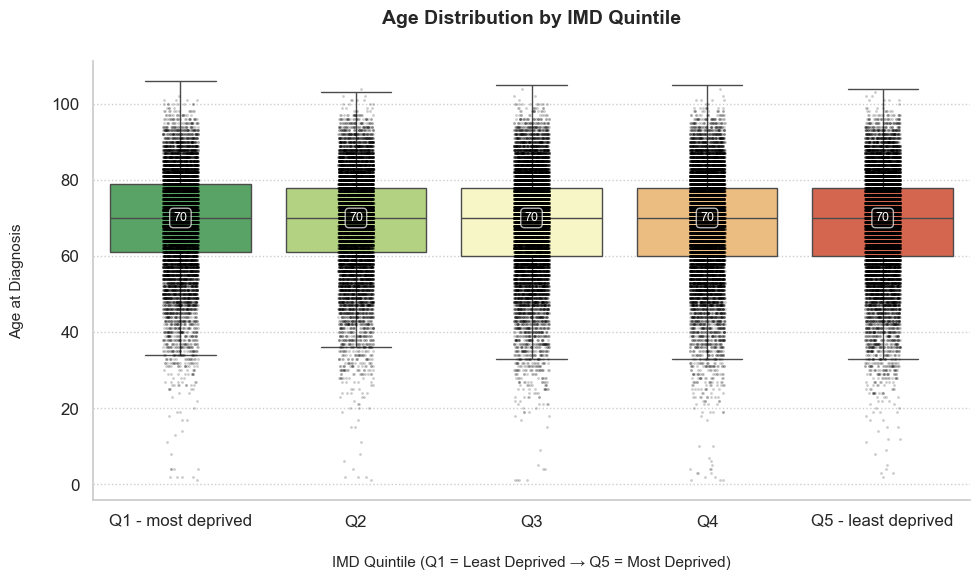
\includegraphics[width=0.83\textwidth, height=0.25\textheight]{Age_Distribution_by_IMD_Quintile.png}
    }
    \caption{Age Distribution By IMD Quintile}
    % \label{fig:age_imd}
    
\end{figure}

Below is the interpretation of the above summary and the chart:-
\begin{itemize}
    \item Having uniform median (as can be seen in the chart) suggests that access of healthcare in terms of age group is relatively equal across different deprivation levels.
    \item The wider range in deprived quintiles suggests disparity in early screening, lifestyle risks.
\end{itemize}



\subsection{Gender Distribution}

Below present are the charts showing distribution of gender (Male, Female) across cancer type and their ratio among themselves i.e., male/female ratio for each deprivation quintile levels.


\begin{figure}[H]
    \centering\fbox{
    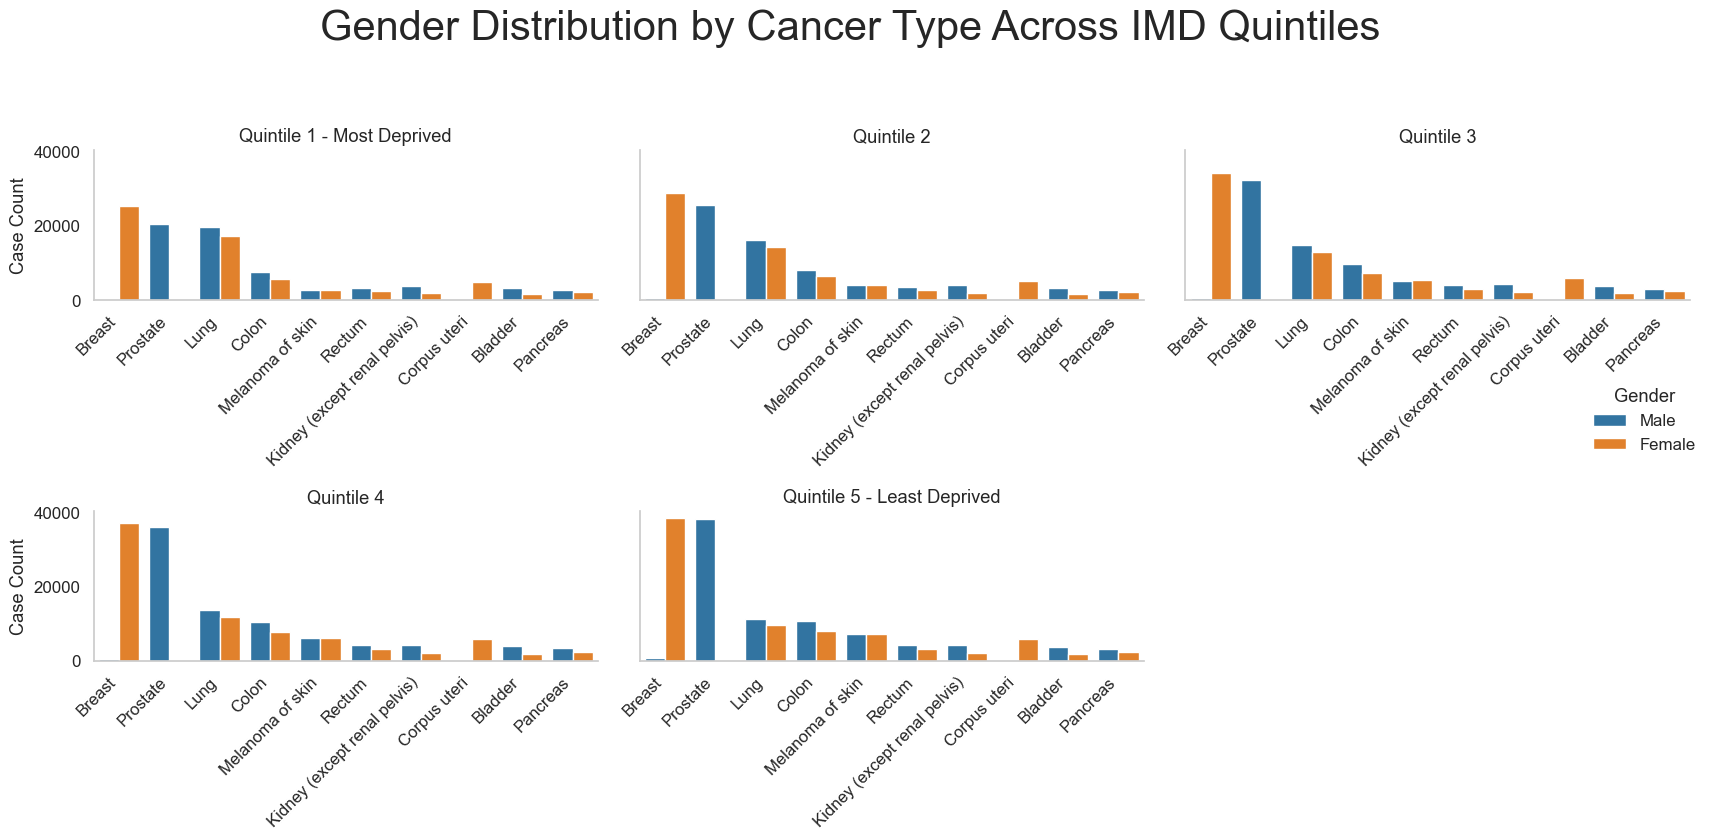
\includegraphics[width=0.83\textwidth]{gender_distribution_by_cancer.png}
    }
    \caption{Gender Distribution By Cancer Type}
    % \label{fig:age_imd}
    
\end{figure}

\begin{figure}[H]
    \centering\fbox{
    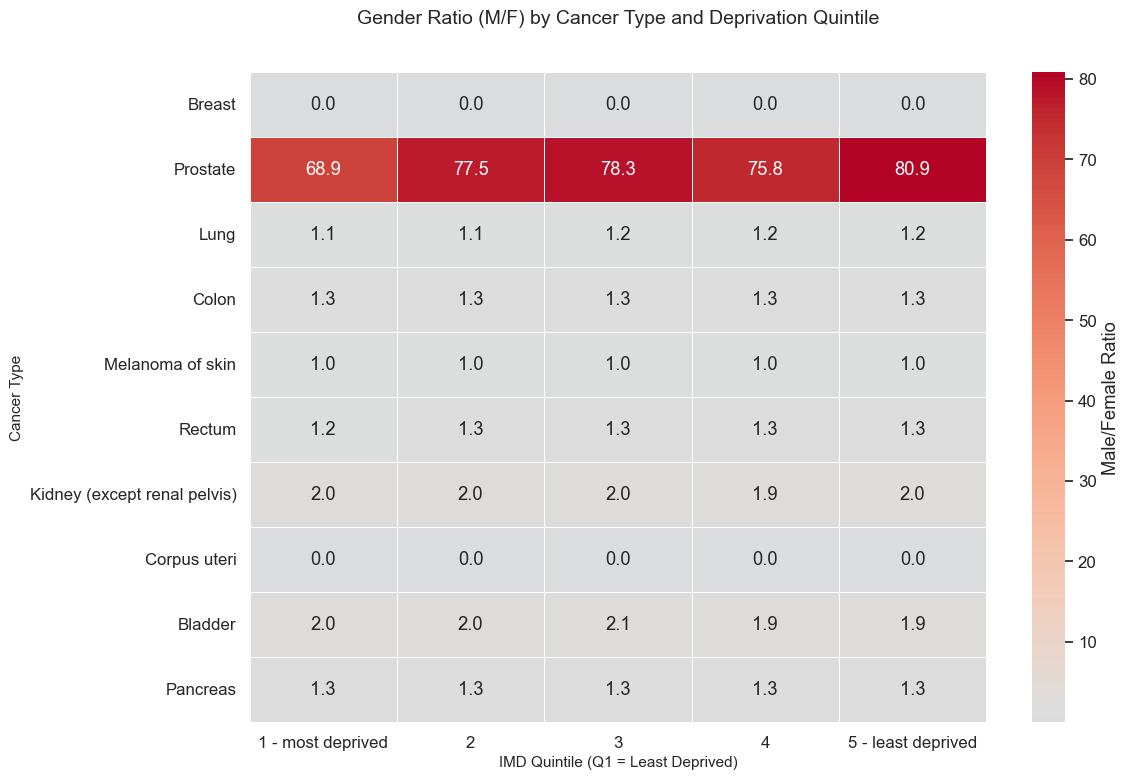
\includegraphics[width=0.83\textwidth, height=0.30\textheight]{gender_ratio_by_cancer_type.png}
    }
    \caption{Gender Distribution By Cancer Type}
    % \label{fig:age_imd}
    
\end{figure}

Based on the charts above are the insights of impact of quintiles at gender level - 
\begin{itemize}
    \item \textbf{Breast Cancer} and \textbf{Corpus Uteri} cases have M/F ratio 0 across all the quintile. That means they are exclusively female cases.
    \item Whereas \textbf{Prostate Cancer} is male dominated disease (where M/F ratio lies between 68 - 81) with slightly higher ration in more deprived quintiles.
    \item \textbf{Lung Cancer} has minimum M/F ratio but has higher overall male incidents (might be due to link with smoking or occupational exposure).
    \item \textbf{Colon, pancreatic and skin melanoma} cancers shows stable M/F ratio across different quintiles, suggesting deprivation does not effect the gender disparity for these cases.
\end{itemize}


% ------------Statistical Analysis Section -----------------
\section{Statistical Analysis}
In this section we will go through some statistical analysis of socioeconomic disparities in cancer epidemiology, addressing three critical dimensions of health inequity. We will apply a multi-method analytical approach to investigate how different factors like age at diagnosis, cancer type, gender and survival outcomes interact with deprivation level using Simulacrum dataset. For this we will be focusing on mainly three issues mentioned below – 
\begin{itemize}
    \item \textbf{Cancer Type Prevalence by Deprivation:}

    We will be using Chi squared test of independence between cancer type and deprivation level and stratified frequency analysis to evaluate whether a specific cancer type shows disproportionate prevalence across the deprivation spectrum. 

    \item \textbf{Age at Diagnosis Patterns}

    Using ANOVA and Kruskal-Wallis test, we will analyze the potential variations in the diagnostic age across different deprivation quintiles. This analysis will help us to find out whether patients in the more deprived areas preset at systematically different ages, which can indicate the disparity in the risk exposure and diagnostic delays.

    \item \textbf{Survival Outcome Disparities}

    To test this, through Kaplan-Meier survival analysis and Cox proportional hazards modeling, will figure out and quantify the differences in the survival rates while adjusting for the clinical and demographic co-variates. This approach enables us to identify independent effect of deprivation on prognosis while controlling for factors like cancer stage and treatment modality.
    
\end{itemize}

This comprehensive approach provides both quantitative evidence and actionable insight for red
using health issues related to cancer in the disadvantaged population. Below are the detailed information of each sections that we have talked about above with methodology, results and discussion for their respective analysis components


\subsection{Cancer Type Prevalence by Deprivation}

\begin{figure}[H]
    \centering \fbox{
    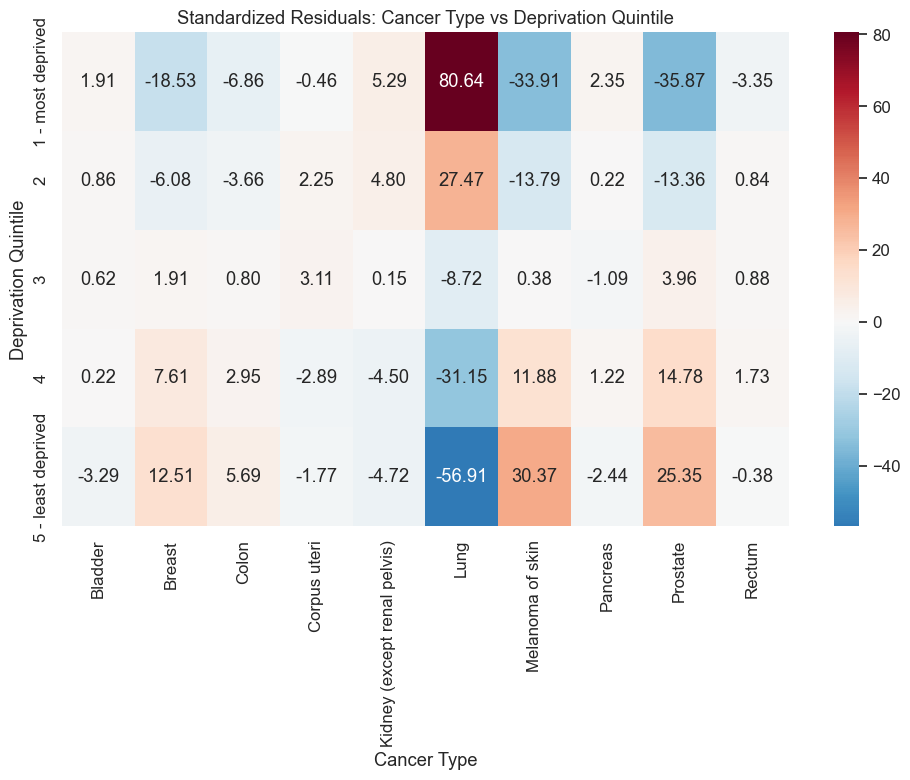
\includegraphics[width=0.9\linewidth,height=0.45\textheight]{Chi_square_test.png}}
    \caption{Standardize Residual: Cancer Type Vs Deprivation Quintile}
    \label{fig:enter-label}
\end{figure}

In this analysis \textbf{Chi Square Test} serves as a primary tool to calculate if cancer type distribution varies drastically across different deprivation quintiles. As it is a non parametric test, it measures discrepancies between observed and expected values/frequencies under null hypothesis and identifies specific disparities via standardized residual. \cite{Agresti2019}

\vspace{1cm} % Vertical space after the paragraph

\textbf{Result:}
\begin{itemize}
    \item Chi-square statistic = 17155.3274, p-value = 0.0000
    \item There is a significant association between cancer type and deprivation level.
\end{itemize}

Based on the chart above it is clearly visible that χ² = 17,155.3274, which shows extreme deviation from expected distribution. While p< 0.0001 indicates that the association is statistically beyond any reasonable doubt. The result validates that deprivation screening should prioritize lung/kidney cancers, and prostrate cancer outreach requires quintile-specific strategy.

% \vspace{0.3cm}

\textbf{Specific Cancer Patterns:}
\begin{itemize}
    \item \textbf{Lung Cancer} shows massive under representation in Q1 (residual = -18.53) and there is over-representation in Q5 (residual = 5.29).
    \item \textbf{Prostate Cancer} shows extreme affluent bias (Q1 residual = 80.64, Q5 residual = -35.87).
\end{itemize}

Thus the result shows that the deprivation effect is clinically meaningful and not just statistically significant. Also, the deprivation effect is heterogeneous across different cancer type.

\subsection{Age at Diagnosis Patterns}
To analyze this, an OLS model was used to examine the factors associated with age during cancer diagnosis. Based on the analysis result present below, it shows statistically significant differences in age across different cancer types. The patients diagnose with cancer types like melanoma and breast cancer are comparatively younger than those with prostate cancer \cite{CancerResearchUK2023}. Additionally, inclusion of gender with cancer in the model confirms that the gender influences age at diagnosis differently across cancer types.

\begin{figure}[H]
    \centering
    \fbox{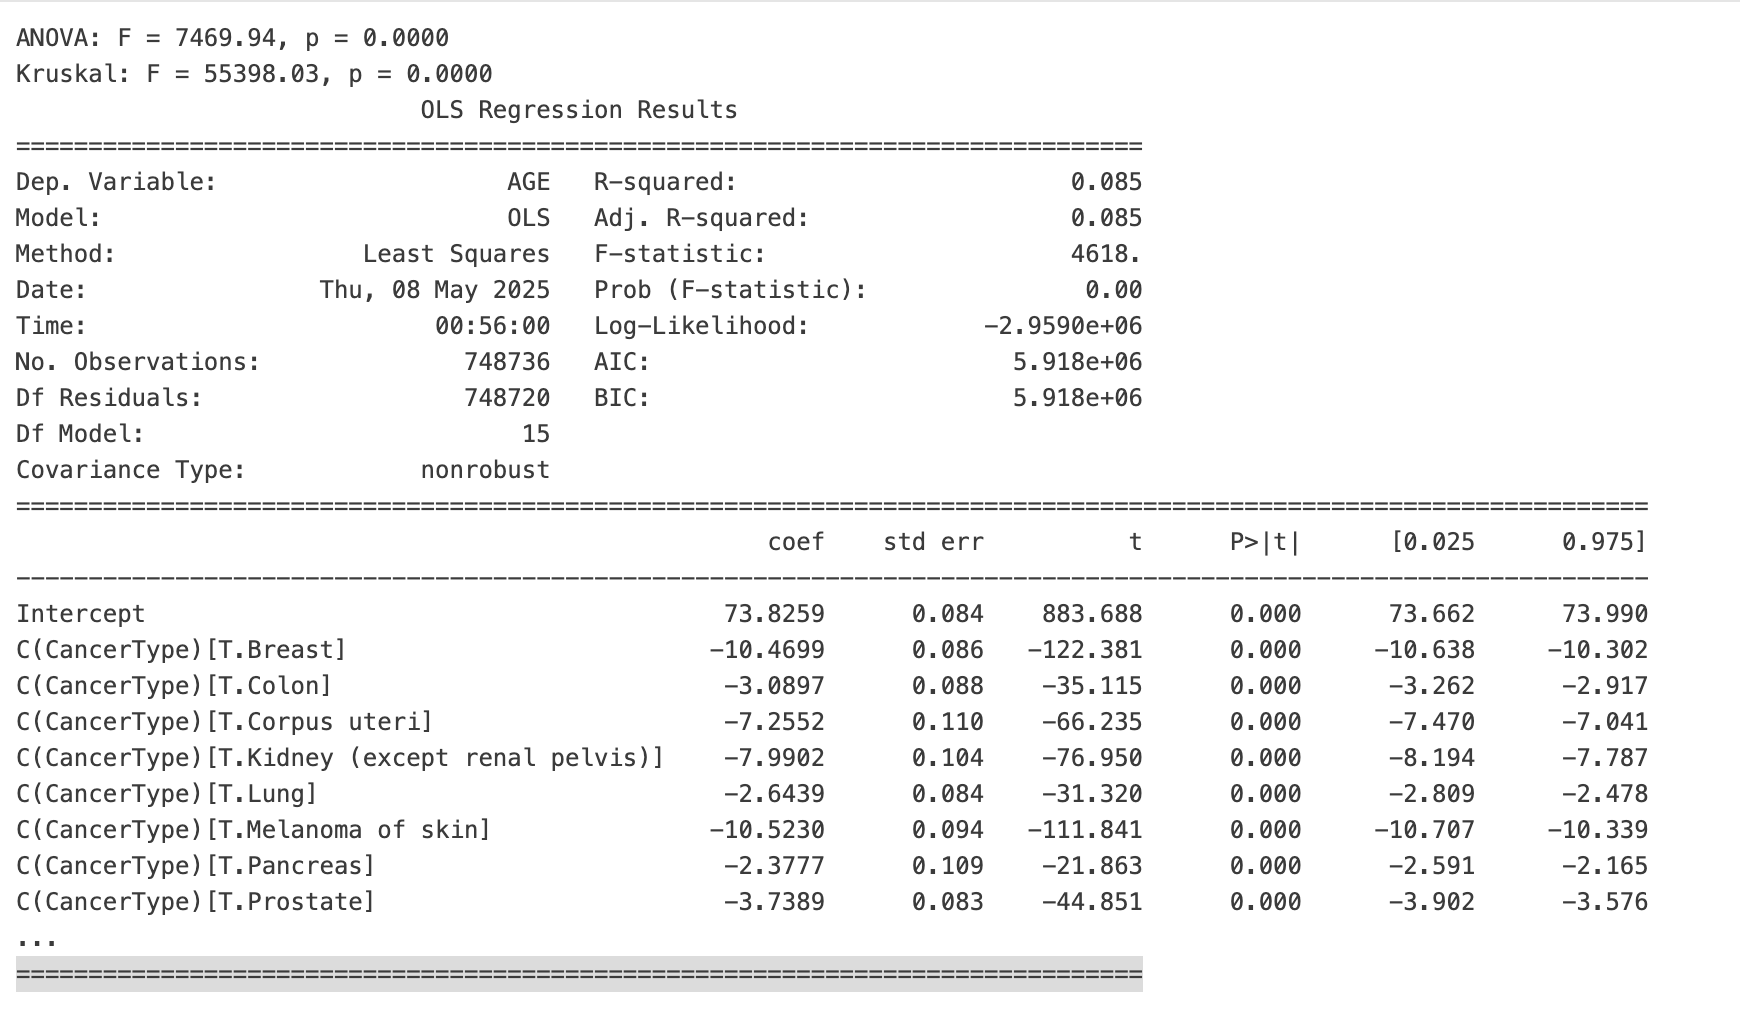
\includegraphics[width=0.90\linewidth]{model_results_age_at_diag.png}}
    \caption{Model Results}
    \label{fig:enter-label}
\end{figure}

Socioeconomic deprivation was also associated with modest but significant difference in diagnosis age consistent with existing literature on healthcare inequalities in UK \cite{PHE2020}. 

% \vspace{0.3cm}
Below are the details about the model and the interpretation of the result: - 

\begin{table}[H]
\centering
\label{tab:variables}
\begin{tabular}{lll}
\toprule
\textbf{Variable} & \textbf{Type} & \textbf{Purpose} \\
\midrule
CancerType & Categorical & To assess how age varies across cancer types \\
GENDER & Categorical & To account for gender differences in age at diagnosis \\
CancerType $\times$ GENDER & Interaction & To allow the effect of gender to vary by cancer type \\
QUINTILE\_2019 & Categorical & To examine age variation across socioeconomic deprivation levels \\
STAGE\_GROUP & Categorical & To control for stage of cancer at diagnosis \\
\bottomrule
\end{tabular}
\caption{Variable Description and Purpose}
\end{table}


\begin{itemize}
    \item \textbf{Cancer Type Matters:-} Each cancer type has statistically significant coefficient. For example, Breast cancer patients on an average diagnosed ~10.5 years earlier than the reference cancer type (intercept group).

    \item \textbf{Gender Differences by Cancer Type:-} The indication terms are significant, confirming that difference of age in male and female varies for each cancer type.

    \item \textbf{Deprivation Level:-}Some quintiles shows statistically drastic variance in age at diagnosis, suggesting that the socioeconomic factor plays minor but measurable role in controlling age at diagnosis after accounting for age and cancer type.
\end{itemize}


\subsection{Survival Outcome Disparities}
Below is the Cox model result for the survival outcome disparity of the cancer patients across different cohorts and in accordance with different geographical and socioeconomic factors.
\begin{figure}[H]
    \centering
    \fbox{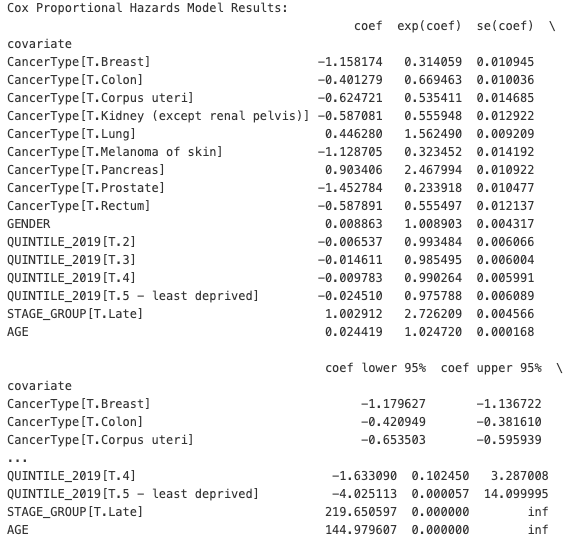
\includegraphics[width=0.6\linewidth, height = 0.35\textheight]{Cox_model_result.png}}
    \caption{Cox model shows survival varies significantly by cancer type, stage, and age}
    \label{fig:enter-label}
\end{figure}

\subsubsection{Survival By Cancer Type}

\begin{figure}[H]
    \centering
    \fbox{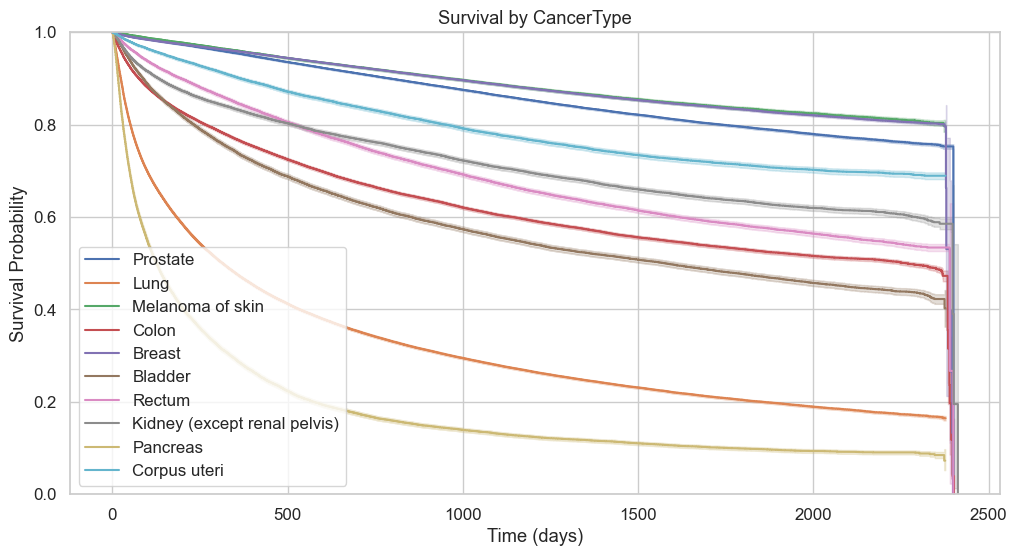
\includegraphics[width=0.8\linewidth]{Survival_by_cancer_type.png}}
    \caption{Kaplan-Meier curves showing variation in survival probabilities across different cancer types}
    \label{fig:enter-label}
\end{figure}
Prostate and Melanoma cancers are showing higher survival probabilities over time with most of the patients surviving over more than 2000 days. Whereas Pancreatic cancer and Lung cancer shows the most declining curve, suggesting higher mortality rate.

Additionally, based on Cox model result- Cancers such as Melanoma (exp(coef) = 0.32), prostate (exp(coef) = 0.23) and breast (exp(coef) = 0.31) cancer has very low hazard ratios, which indicates better survival rate for this. Whereas Pancreatic and lung cancer have increased hazard ratios, which also confirms the result from Kaplan-Mier result.

\subsubsection{Survival By Deprivation Quintile}
        
\begin{figure}[H]
    \centering
    \fbox{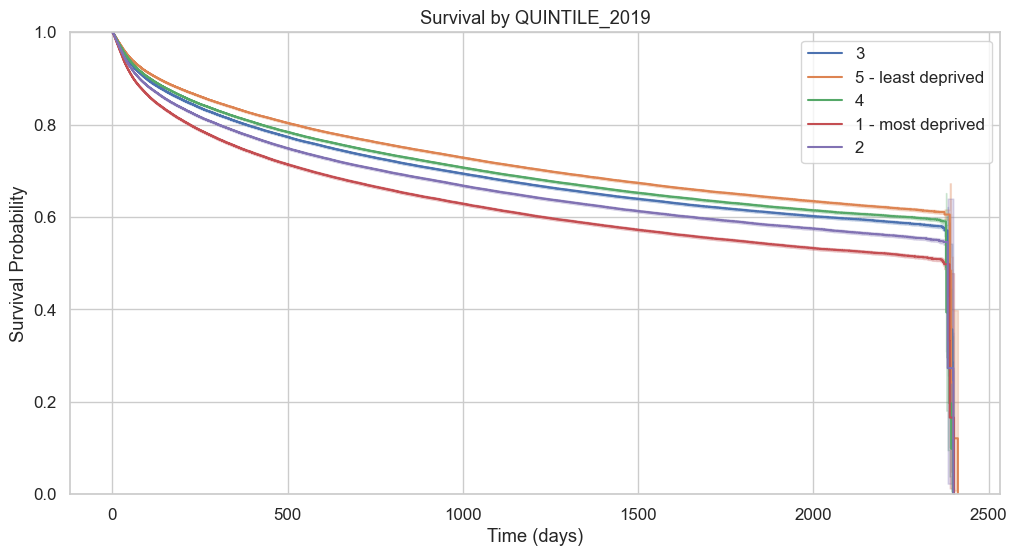
\includegraphics[width=0.8\linewidth]{Survival_by_Deprivation.png}}
    \caption{Survival probability by gender over time}
    \label{fig:enter-label}
\end{figure}
The above results confirms that socioeconomic deprivation is inversely proportional to the survival rate, even here the the gap in curves grows higher with time.

The Cox model shows a bit of positive effect with decreasing deprivation. Quintile 5 has hazard ratio of 0.976, means approximately 2.4$\%$ of reduction in risk of death.
\subsubsection{Survival By Gender}

\begin{figure}[H]
    \centering
    \fbox{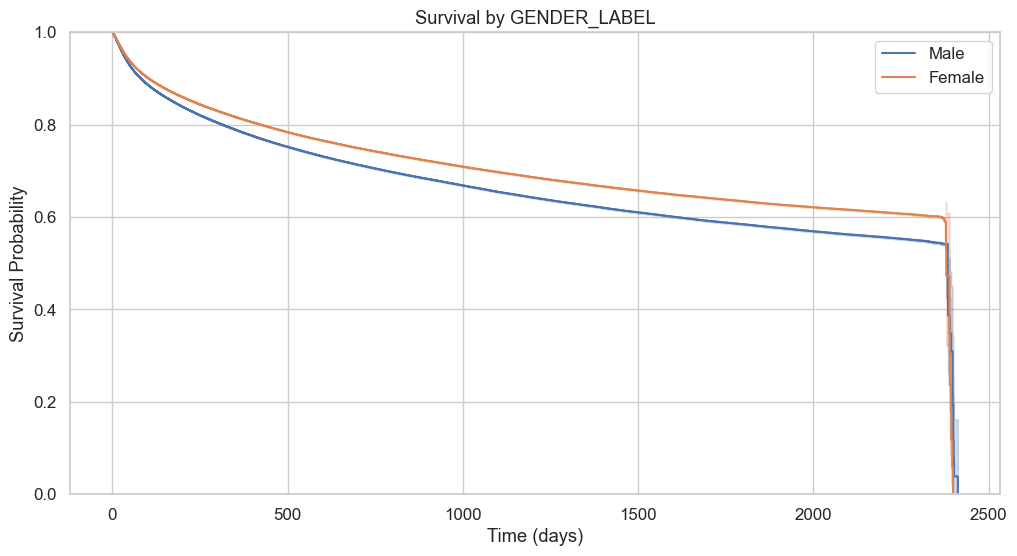
\includegraphics[width=0.8\linewidth]{Survival_by_gender.png}}
    \caption{Survival outcomes by socioeconomic deprivation level}
    \label{fig:enter-label}
\end{figure}
Based on the result above we can see that females have better survival rate as compared to men across entire observation period and the separation grows with time. This disparity could be due to biological factor, healthcare access and health-seeking behavior.

However Cox model coefficient for Male is very low but positive(exp(coef) = 1.009) suggesting males has very marginal increase in hazard. Though the p-value (p<0.05) is very significant it has minimal impact as compared to gender and cancer types.


% ------------Conclusion Section -----------------
\clearpage
\section{Conclusion}
Based on all the analysis that we did in the previous sections the results shows significant disparities in the cancer outcomes and diagnostic patterns, influenced by many different variables/parameters like cancer type, age, gender, stage etc.,. Using these models results we can say that cancer type and stage at diagnosis are one of the strongest predictor of survival. Patients suffering from pancreatic cancer and lung cancer has the highest mortality risks, whereas melanoma and breast cancers have higher survival rate.

When looking at the gender disparities in survival, females shows slightly better outcomes than males. Though the socioeconomic deprivations are less pronounced, they shows consistent influence. Patients from the most deprived quintiles (Q5) shows slightly higher risk of death as compared to the lower deprived quintiles, indicating inequality in healthcare access still remains a concern for them.

Additionally, while deep diving into age at diagnosis, the linear regression shows a complex relationship between socioeconomic factors and diagnostic timings. Patients from different deprived quintiles are diagnosed at different ages, specially for the most deprived section. Notably, the breast cancer patients are diagnosed approximately 10.5 years earlier than the reference group. 

At the end, collectively all these results confirms that the deprivation effects in various cohorts are clinically meaningful and heterogeneous across different cancer types. Which specifies the need of targeted public health strategies to be implemented across the country, which includes earlier screening in the most deprived quintile communities and setup the system in a way to customize the outreach program based on socioeconomic profiles and cancer specific disparities.
% ------------Reference Section -----------------

\clearpage  % Forces a new page
\bibliographystyle{plain}
\bibliography{references}
\clearpage
\begin{figure}
    \centering
    
\includegraphics[width=1.0\linewidth]{Academic Integrity.png}
    \label{fig:enter-label}
\end{figure}
\end{document}